\section{\bfseries Predlog korisničkog interfejsa}

U ovom poglavlju će biti prikazan zamišljen izgled korisničkog interfejsa ove aplikacije. Aplikaciju koriste zaposleni kao i korisnici. U narednim podsekcijama biće prikazane slike određenih delova aplikacije uz kratko objašnjenje.

\subsection{\bfseries Registrovanje korisnika}

Način registrovanja korisnika je prikazan na slici \ref{fig:Registrovanje korisnika}. Registrovanje se sastoji od unošenja korisničkog imena, mejla i lozinke.  Izvršava se klikom na dugme \say{Sign Up}. Registrovani korisnik može klikom na dugme \say{Sign in} da se prijavi kao što je objašnjeno u sekciji \ref{Prijavljivanje_korisnika_sekcija}.

\begin{figure}[H]
\begin{center}
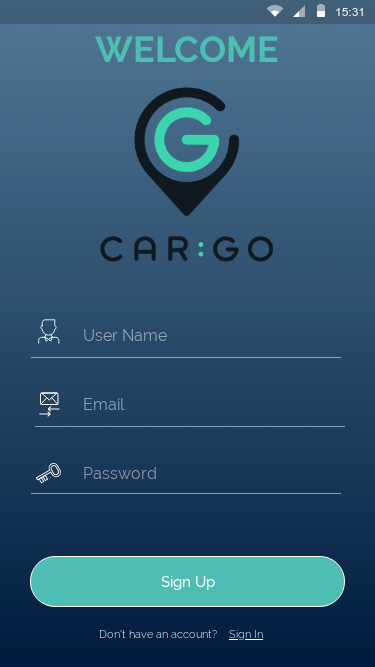
\includegraphics[width=4cm]{Slike/Registrovanje.png}
\end{center}
    \caption{Registrovanje korisnika}
\label{fig:Registrovanje korisnika}
\end{figure}

\subsection{\bfseries Prijavljivanje korisnika}
\label{Prijavljivanje_korisnika_sekcija}

Prijavljivanje korisnika (slika \ref{fig:Prijavljivanje korisnika}) koristi postojeće korisničko ime i lozinku. Prijavljivanje se izvršava klikom na dugme \say{Sign In} nakon ispravno unešenog korisničkog imena i lozinke.
\begin{figure}[H]
\begin{center}
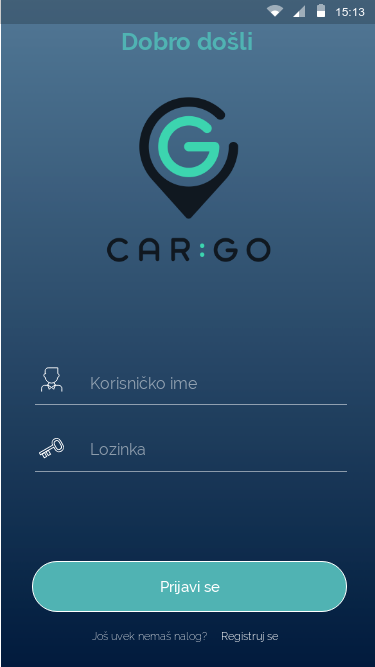
\includegraphics[width=4cm]{Slike/Prijavljivanje.png}
\end{center}
    \caption{Prijavljivanje korisnika}
\label{fig:Prijavljivanje korisnika}
\end{figure}


\subsection{\bfseries Profil korisnika}

Nakon uspešnog prijavljivanja na svoj nalog, korisniku se prikazuje prva strana (slika \ref{fig:Profil korisnika}) na kojoj korisnik može da naruči vožnju, podesi informacije o kreditnoj kartici i da se odjavi. Klikom na dugme \say{Podešavanja kreditne kartice} korisniku se otvara nov prozor (slika \ref{fig:Podešavanje kartice}) u koji treba uneti sve potrebne informacije o kartici kako bi plaćanje moglo da bude realizovano. Ukoliko se klikne na dugme \say{Naručivanje vožnje} otvara se novi prozor u kome korisnik može da naruči vožnju (videti sekciju \ref{Naručivanje vožnje}).


\begin{figure}[h!]
\centering
\begin{minipage}{.5\textwidth}
  \centering
  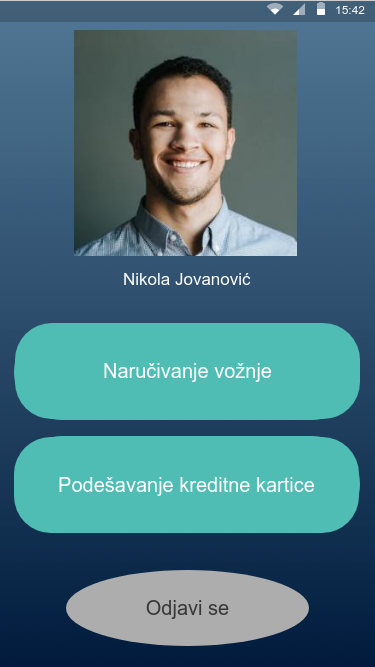
\includegraphics[width=.4\linewidth]{Slike/Profil.png}
  \caption{Profil korisnika}
  \label{fig:Profil korisnika}
\end{minipage}%
\begin{minipage}{.5\textwidth}
  \centering
  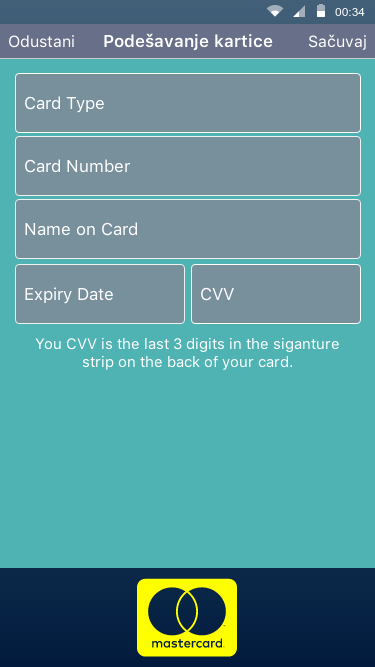
\includegraphics[width=.4\linewidth]{Slike/upravljanje_karticom.png}
   \caption{Podešavanje kartice}{}
  \label{fig:Podešavanje kartice}
\end{minipage}
\end{figure}


\subsection{\bfseries Naručivanje vožnje}
\label{Naručivanje vožnje}

Za naručivanje vožnje, korisniku je omogućeno da unese željenu lokaciju (slika \ref{fig:Naručivanje vožnje}). Nakon toga, aplikacija mu omogućava da vidi cenu vožnje klikom na dugme \say{Procenjena cena} (slika \ref{fig:Procena cene}).


\begin{figure}[H]
\centering
\begin{minipage}{.5\textwidth}
  \centering
  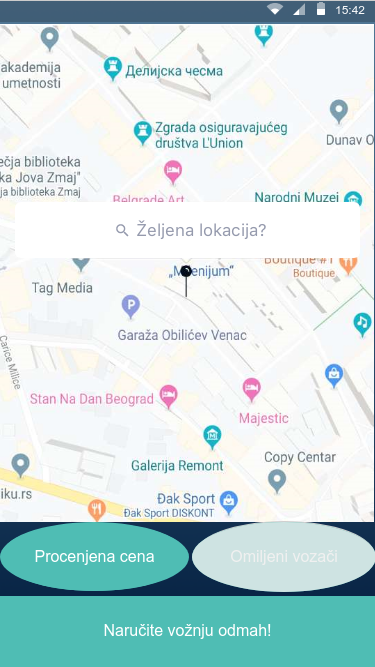
\includegraphics[width=.4\linewidth]{Slike/Narucivanje_sa_adresom.png}
  \caption{Naručivanje vožnje}{}
  \label{fig:Naručivanje vožnje}
\end{minipage}%
\begin{minipage}{.5\textwidth}
  \centering
  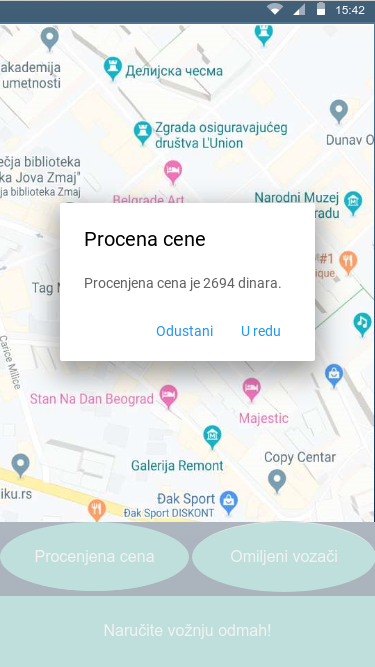
\includegraphics[width=.4\linewidth]{Slike/Procena_cene.png}
   \caption{Procena cene}{}
  \label{fig:Procena cene}
\end{minipage}
\end{figure}

Kada korisnik klikne na \say{Naručite vožnju odmah} vrši se pretraga slobodnih vozača najbiližih trenutnoj lokaciji korisnika (slika \ref{fig:Pronalazenje vozaca}). U ovoj fazi korisnik može prekinuti pretragu klikom na \say{Odustani} ukoliko se predomisli i više ne želi vožnju.

\begin{figure}[H]
\begin{center}
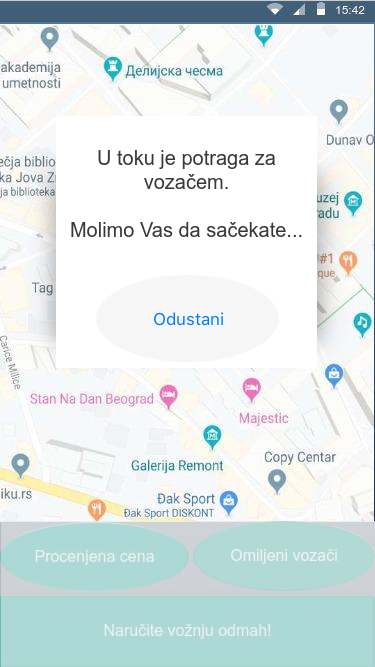
\includegraphics[width=4cm]{Slike/Pronalazenje_vozaca.png}
\end{center}
    \caption{Pronalaženje vozača}
\label{fig:Pronalazenje vozaca}
\end{figure}


Kada se završi pretraga korisnik dobija listu svih pogodnih vozača i bira onog kog želi (slike \ref{fig:Vozaci na raspolaganju} i \ref{fig:Prihvacena voznja}).

\begin{figure}[H]
\centering
\begin{minipage}{.5\textwidth}
  \centering
  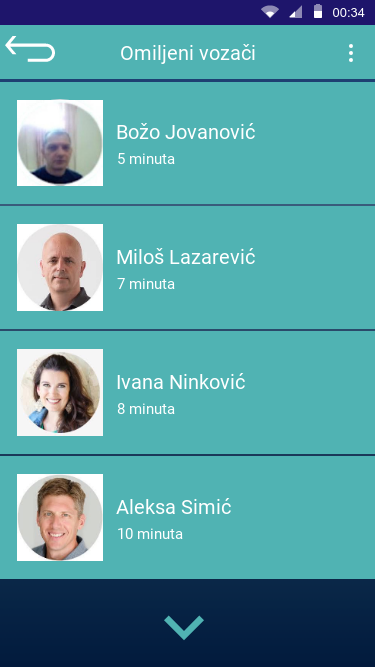
\includegraphics[width=.4\linewidth]{Slike/vozaci_na_raspolaganju.png}
  \caption{Vozači na raspolaganju}
  \label{fig:Vozaci na raspolaganju}
\end{minipage}%
\begin{minipage}{.5\textwidth}
  \centering
  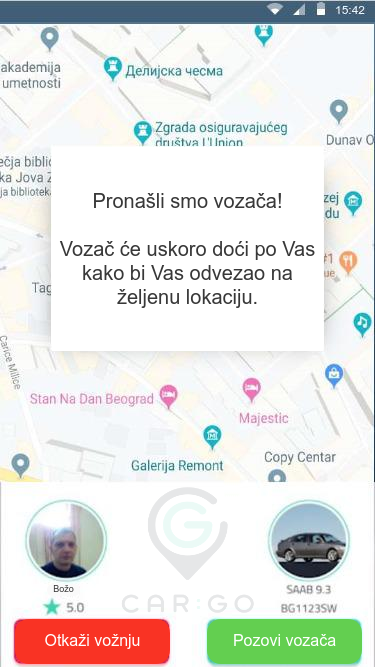
\includegraphics[width=.4\linewidth]{Slike/Prihvacena_voznja.png}
   \caption{Prihvaćena vožnja}
   \label{fig:Prihvacena voznja}
\end{minipage}
\end{figure}

\newpage

\subsection{\bfseries Završetak vožnje}

Nakon završene vožnje sistem nudi korisniku mogućnost da oceni i napiše neki komentar o vozaču ukoliko to želi (slika \ref{fig:Ocenjivanje vozaca}).

\begin{figure}[h!]
\begin{center}
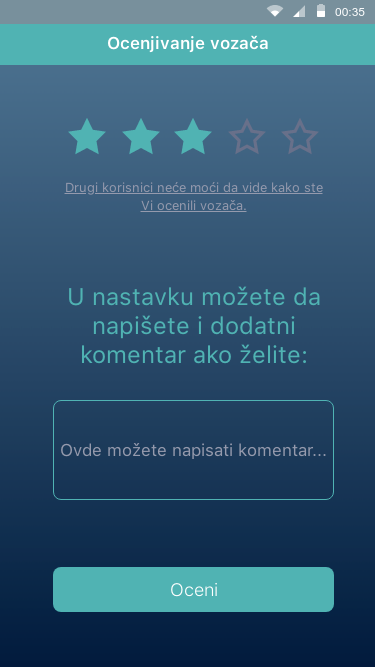
\includegraphics[width=4cm]{Slike/ocenjivanje_vozaca.png}
\end{center}
    \caption{Ocenjivanje vozača}
\label{fig:Ocenjivanje vozaca}
\end{figure}













